\documentclass[12pt]{amsart}
\usepackage[margin=1in]{geometry}
\usepackage{fancyhdr}

\pagestyle{empty}

\usepackage{amsmath}
\usepackage{amssymb}
\usepackage{amsthm}
\usepackage{enumerate}
\usepackage{color}
\usepackage{graphicx}

\usepackage{hyperref}
\hypersetup{
    colorlinks=true,
    linkcolor=blue,
    filecolor=magenta,      
    urlcolor=blue,
    citecolor=blue,
}

\newcommand{\mk}{\textsf{M\&K}}
\newcommand{\con}{\textsf{CON}}
\newcommand{\sts}{\textit{Slay the Spire}}

\newcommand{\red}[1]{\textcolor{red}{#1}}
\newcommand{\blue}[1]{\textcolor{blue}{#1}}
\newcommand{\green}[1]{\textcolor{green}{#1}}
\newcommand{\magenta}[1]{\textcolor{magenta}{#1}}


\newtheorem{question}{Question}

\lhead{}
\rhead{}
\pagestyle{fancy}
\begin{document}

\begin{center}
    \Huge Speedrunning tricks in \textit{Slay the Spire}
\end{center}

\thispagestyle{plain}

\tableofcontents

\section{Why make this document? }
Many tricks are covered in video tutorials made by members of the \textit{Slay the Spire} speedrunner community.  
On the other hand, some strategies are a work-in-progress. 
Our intent here is to capture new exploits and organize them in a pdf-readable fashion which supplements and hyperlinks to, but does not replace, other speedrun resources.  
This gives us organized information to share with new members of our community which can be easily updated when we make new developments. 
\cite{ForgottenArbiterMoreGlitches}


\section{Getting started}
To speedrun ~\sts, all you need is a legal file setup and a method of recording and timing your runs (we strongly suggest LiveSplit and the built-in autosplitter).  
You should consider the many speedrunning categories on the \textrm{Speedrun.com} leaderboards \cite{SlayTheSpireLeaderboards} and decide for yourself which ones you would like to try.  
You can even try unofficial speedrun categories that you enjoy, which can also be of interest to the speedrunner community.  
\subsection{Legal file setups}
To speedrun \sts~, your game files need to be in a state that can be obtained through normal play.  
Normal play comprises of anything that can be done within the game that would be considered legal when speedrunning.  
For example, runs can be legally ended when they are won, lost, abandoned while in play, or abandoned from the main menu.  
Any glitches or exploits which are legal for a run can also used when making a legal file setup yourself.  
On the other hand, editing game files arbitrarily is strictly prohibited.  
\\

When attempting runs, you may progress unlocks unfavorably.  
To alleviate the burden of repeatedly progressing from a fresh save file, most runners will simply edit the contents of their \textrm{preferences} folder to a desirable legal state.  
 legally achieve a correct setup, you can also paste the contents of legal \textrm{preferences} folder into your game's \textrm{preferences}.  
This can be done while the game is running as long as you open another save file from within the game and re-enter the save file where you plan to speedrun.  
This way, you avoid having to close your game at any point.  
Be sure to abandon any saves that are in the middle of a run to avoid any accidental illegal unlocks.  \\

To avoid having to manually copy and paste game files, you can instead use scripts that do this work for you.  
See Phantom's guide \cite{PhantomPreferences} for a description and helpful tutorial.  
This approach works well for many runners.  
Note that this guide claims that the game must be closed, but in fact it is also sufficient to enter another game file and and re-entering the desired game file after modifying the \textrm{preferences} folder.  

\subsection{How unlocks work}
The most important aspects of a file setup are the unlocks: 
\begin{enumerate}
	\item 
		\textbf{Character unlocks. }
		From a new save file, the Silent can be unlocked by starting a run with the Ironclad and immediately abandoning.  
		The Defect unlocks by similarly starting and abandoning with the Silent.  
		For the Watcher, unlock the Silent and Defect, and win a run with any class.  
		Specifically, this requires defeating the Act III boss without abandoning prematurely.  
	\item 
		\textbf{Class unlocks. }
		Each class has $5$ levels of unlocks that are based on accumulated score for that class.  
		These unlocks consist of an assortment of relics which are either class-specific or available to all classes, and cards which are specific to the given class.  
	\item 
		\textbf{Bosses seen. }
		From a new save file, the game is coded to ensure that the player encounters the Act I, II, and III bosses for the first time in a specific order.  
		For Act I: Guardian, Hexaghost, and Slime Boss.  
		For Act II: Champ, Bronze Automaton, and Collector.  
		For Act III: Awakened One, Time Eater, and Donu \& Deca.  
		If all $3$ bosses from an Act have been seen by the player, a boss determined by the run's seed will instead be generated.  
	\item 
		\textbf{Neow Bonuses. }
		On each class, the player earns a choic of $4$ starting bonuses from Neow on floor $0$ if the previous run reached $16$, the floor which corresponds to the Act I boss.  
		If the player did not reach this floor on their previous run with the given class, then Neow instead offers Neow's Lament or a fixed amount of max HP.  
	\item 
		\textbf{Ascension level.  }
		On each class, if the player defeats the Act III boss on the their highest Ascension level (except Ascension $20$), then the next Ascension level is unlocked.  
\end{enumerate}

There are some nuances to these unlock conditions that should be addressed.  
First, the character unlocks, class unlocks (and accumulated score), and Ascension levels are only updated in the post-run screens, but not when a run is abandoned from the game's main menu.  
On the other hand, a boss is ``seen'' the instant that the player enters a combat with that boss for the first time, and there is no check based on any other factor (e.g., floor number, if the boss is defeated, or how the run ends).  
On the other hand, the player earns the $4$-option Neow bonus simply by reaching floor $\#16$ and no other checks are made (e.g., the type of map node the player visits, whether the player has seen the Act I boss, or how the run ends).  

\subsection{Optimal file setups}
With the wrong file setup, you will struggle to find cards and relics that make your runs fast and consistent.  
First, be aware of the class unlocks which are organized in Figure \ref{fig: class unlocks}.  
\begin{figure}[h]
\begin{tabular}{l|l}
Ironclad     &                                             \\ \hline
Unlock \#$1$ & Heavy Blade, Spot Weakness, Limit Break     \\
Unlock \#$2$ & \magenta{Omamori}, \magenta{Prayer Wheel}, \magenta{Shovel}               \\
Unlock \#$3$ & Wild Strike, Evolve, Immolate               \\
Unlock \#$4$ & Havoc, Sentinel, Exhume                     \\
Unlock \#$5$ & \magenta{Blue Candle}, \magenta{Dead Branch}, \magenta{Singing Bowl}      \\ \\
Silent       &                                             \\ \hline
Unlock \#$1$ & Bane, Catalyst, Corpse Explosion            \\
Unlock \#$2$ & \magenta{Du-Vu Doll}, \magenta{Smiling Mash}, \magenta{Tiny Chest}        \\
Unlock \#$3$ & Cloak and Dagger, Accuracy, Storm of Steel  \\
Unlock \#$4$ & \magenta{Art of War}, \magenta{The Courier}, \textbf{\magenta{Pandora's Box}}      \\
Unlock \#$5$ & Concentrate, Setup, \textbf{Grand Finale}            \\ \\
Defect       &                                             \\ \hline
Unlock \#$1$ & Rebound, Equilibrium, Echo Form             \\
Unlock \#$2$ & TURBO, Sunder, Meteor Strike                \\
Unlock \#$3$ & \textbf{Hyperbeam}, Recycle, Core Surge              \\
Unlock \#$4$ & Gold-Plated Cables, \magenta{Turnip}, Runic Capacitor \\
Unlock \#$5$ & Data Disk, Symbiotic Virus, Emotion Chip    \\ \\
Watcher      &                                             \\ \hline
Unlock \#$1$ & Prostrate, \textbf{Blasphemy}, Devotion              \\
Unlock \#$2$ & Foreign Influence, Alpha, Mental Fortress   \\
Unlock \#$3$ & Spirit Shield, Wish, Foresight              \\
Unlock \#$4$ & \textbf{\magenta{Akabeko}}, Duality, \magenta{Ceramic Fish}              \\
Unlock \#$5$ & Strike Dummy, Teardrop Locket, Cloak Clasp 
\end{tabular}
    \caption{
        All unlocks, by class.  
        Relics marked in magenta are not class-specific.  
        Notable unlocks are bold-faced.  
    }
    \label{fig: class unlocks}
\end{figure}
~\\
The bosses appear to the player in a fixed order.  
In Any\%, the player can set up their file in a legal fashion to meet the desired bosses.  
The fastest boss is in bold, with the exception of Watcher preferring Timer Eater.  
\begin{itemize}
    \item Act I: Guardian, Hexaghost, \textbf{Slime Boss}.  
    \item Act II: Champ, Bronze Automaton, \textbf{Collector}.  
    \item Act III: Awakened One, \textbf{Donu \& Deca}, Timer Eater* (Watcher).  
\end{itemize}

For convenience, we will describe unlocks using a string of the form ``Unlocks: *,*,*,*; Bosses: *,*,*''
Each ``*'' will be replaced with a number or set of numbers which indicate unlock levels by class (ordered Ironclad, Silent, Defect, and Watcher) and the number of bosses seen in each Act.  
Based on the current Any\% world records and community consensus, the suggested Any\% unseeded setups are: 
\begin{itemize}
    \item 
        \textbf{Ironclad.  }
        Unlocks: 
            $0, 
            \{4,5\}, 
            \{0,1,2,3\}, 
            4$. 
        Bosses: 
            $2, 
            2, 
            1$.  
    \item 
        \textbf{Silent.  }
        Unlocks: 
            $\{0, 1\}, 
            5, 
            \{0, 1, 2, 3\}, 
            \{0, 1, 2, 3\}$.  
        Bosses: 
            $2, 
            2, 
            1$.  
    \item 
        \textbf{Defect.  }
        Unlocks: 
            $\{0, 1\}, 
            \{4, 5\}, 
            3, 
            \{0, 1, 2, 3\}$.  
        Bosses: 
            $2, 
            2, 
            1$.  
    \item 
        \textbf{Watcher.  }
        Unlocks:
            $\{0, 1\}, 
            \{4, 5\}, 
            \{0, 1, 2, 3\}, 
            4$.  
        Bosses: 
            $2, 
            2, 
            2$.  
\end{itemize}
\subsection{Game settings}
Finally we will conclude this section with a discussion of the game settings.  
The optimal game settings that affect speed are largely unambiguous.  
Set \textbf{max framerate} to the highest value and enable \textbf{fast mode}, disable \textbf{screenshake}, \textbf{VSync}, \textbf{confirmation when choosing $1$ card}, and \textbf{particle effects}.  
See Figure \ref{fig: game settings}.  
\begin{figure}[h]
    \centering
    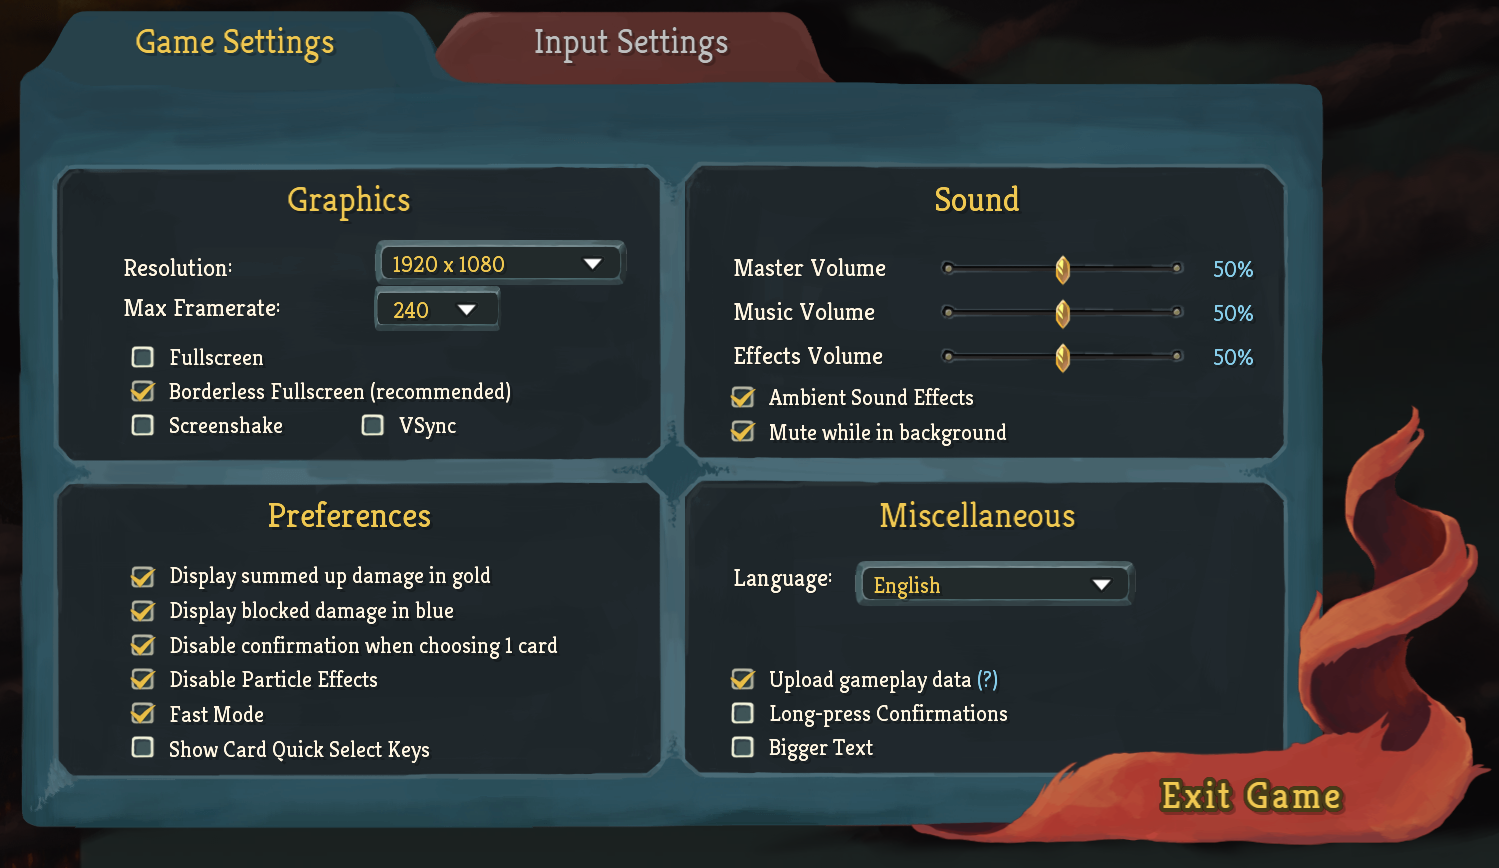
\includegraphics[scale=.25]{graphics/GameSettings.PNG}
    \caption{An example of speedrun-friendly game settings.  }
    \label{fig: game settings}
\end{figure}

\section{Input methods}\label{sec: input methods}
\sts~is coded to accommodate mouse and keyboard (\mk) and controller (\con) use.  
Controller use in \sts~speedruns is fairly new and resources on its use are not as widely developed.  
While \mk~is the most comfortable input method for most speedrunners, there are benefits to having a controller plugged in so you can temporarily use it in certain situations.  
After using \con, the player must click a mouse button before being able to properly operate a mouse.  
Left-clicking will select any option that is highlighted by the controller selections, right clicking will ``examine'' cards selected in shops, and scroll wheel clicking makes no actions.  
\\

It is important to emphasize that the ``hybrid'' approach (repeated switching between \mk~and \con) is mainly relevant to runners who are attempting world records and not recommended for new players.  
The player should not expect to save more than $15$ seconds on unseeded runs, even under ideal conditions. 
For new players, it is significantly more important to master other aspects of speedrunning \sts~such as fast inputs and good routing, card play, potion use, card choices, relic purchases, and event decisions.  
Mistakes on \con~ very easily result in: 
\begin{itemize}
    \item run-ending map node selections.  
    \item time-loss or misclicks when switching input methods, unpracticed.  
    \item accidental discarding of potions.  
\end{itemize}

Ultimately the runner's discretion will determine how far they are willing to go.  
\\

In this section, we will discuss situations where \con~enhances \mk~play and situations where it detracts.  
Then we will discuss keyboard and button layouts.  
\subsection{Input methods in different scenarios}
In this section, we will assume that you normally use \mk~as your preferred input method.  
For the glitches mentioned, see Section \ref{sec: glitches and exploits} for more details.  
Here we way input methods in different in-game scenarios: 
\begin{itemize}
	\item 
	    \textbf{Events.  }
	        \con~ is mostly faster than \mk.  
	\begin{enumerate}[-]
		\item 
			The main reason for this is that using \con, subsequent event menus are interactable instantly and do not require moving and accurately clicking with a mouse cursor.  
			Tbe time save is especially noticeable in the Scrap Ooze and Cursed Tome events where mashing `select' makes short work the event.  
	    \item 
	        Using \con, the player can prevent curses, Bites, etc from being added to the deck during events (see Section \ref{sub-sec: card skips}).  
	        It can be especially helpful to already have a controller in hand to save the time of switching to controller.  
		\item 
		    Using \con, events with complicated card selection menus must be handled with care on controller when the number of cards is not a multiple of $5$.  
		    For example, pressing `up' to select a card to be removed/upgraded/transformed with $9$ cards available will take the player to the second-to-last card.  
		    This mechanic hasn't been fully investigated by the community, but it is easy to plan around in seeded runs.  
	\end{enumerate}
	\item 
	    \textbf{Combats.  }
		\mk~outperforms \con~significantly.  
		\begin{enumerate}[-]
			\item 
			    On \mk, card number shortcuts and mouse clicks make it easy to select and play cards and to target enemies.  
			    The mouse also makes it easy to play multiple potions in succession, with the only possible exception being the potions which require targeting an enemy and clicking.  
			    This can be overcome in certain fights in seeded runs.  
		\item 
		    It is worth noting that using \con, after a card is queued to play, the card to the right (wrapping around) is selected next.  
		\item 
		    On \con, for a few frames at the star of combat, any combat-only potion defaults to the `discard' option.  
		    Additionally, the potion panel does not wrap around and the empty slots occupy space.  
		    As with \mk, cards cannot be selected prematurely during their draw animation.  
		    For this reason, moving `left' from first position during the draw animation takes the player to the last card selectable, not the last card being drawn.  
		\end{enumerate}
	\item 
		\textbf{Shops.  }
		\mk~outperforms \con~when purchasing at shops.  
		\begin{enumerate}[-]
		    \item 
		        Using \mk, it is very easy to purchase relics, potions, and make removals.  
		        On \con, any purchase takes the player to the top-left-most selection.  
	        \item 
	            On \con during the few frames of the `enter shop' animation, the colorless card in the bottom-left is the first selection.  
	            After a few more frame, selection returns to the top-left card.  
	            This happens during the `enter shop' animation because of the options which are on-screen and thus selectable.  
		\end{enumerate}
	\item 
        \textbf{Map pathing.  }
        \con~can outperforms or is otherwise on path with \mk.  
        \begin{enumerate}[-]
            \item 
                Using \con~ comes with the very real risk of mis-pathing.  
            \item 
                Using \con, the selection defaults to the middle-most or middle-right node.  
                For example, the defaults are node $\#2$ of $2$, $\#2$ of $3$, $\#3$ of $5$, etc.  
            \item 
                Node buffering (e.g., $2$-node, $N$-node, and Necronomicurse skip) may be easier to perform to some players on $\con$.  
                See Section \ref{sub-sec: node buffering}.  
        \end{enumerate}
    \item 
        \textbf{Rest sites.  }
        \con~ is slightly faster \mk~when spamming `rest', the default selection.  
        \begin{enumerate}[-]
            \item 
                When smithing, one input method may be faster than the other due to the card selection menu.  
        \end{enumerate}
\end{itemize}

\subsection{Keyboard and button layouts}
The input settings for \mk~ require very few tweaks for most runners.  
The most crucial change is the choice of a `map' key.  
For example, \textbf{Q} is easily reachable from the number keys (which are the fastest way to select cards in combat) and from a \textbf{WASD} hand position. 
Also, \textbf{Z} or other surrounding keys are close to \textbf{WASD}.  
Alternatively, \textbf{Space} can also be used for the `map' key due to it's size.  \\

For controllers (\con), the story is quite different.  
First consider the following: 
\begin{itemize}
    \item 
        When node buffering or card skipping, (see Sections \ref{sub-sec: node buffering} and \ref{sub-sec: card skips}), the player must take care to select the correct node when the default node is not desired.  
    \item 
        There are two defaults for directional movements (D-pad and left thumbstick).  
        The game will not register two directional movements on the same frame.  
    \item 
       The default `Proceed/End Turn' button is opposite the default `Select' button, which is not ideal for mashing.  
    \item 
        In speedruns, the player almost never wants to check their draw pile, discard pile, exhaust pile, and deck.  
        For this reason, these buttons should be remapped to buttons that are less accessible.  
    \item 
        Especially in seeded speedruns, the `cancel' button is unhelpful to press and should also be mapped to something less easily pressed.  
\end{itemize}
In Figure \ref{fig: controller layout}, we show an example of a speedrun-friendly button layout.  
Here, we have remapped unwanted selections to the center-thumbstick clicks, bumper buttons, and right thumbstick to avoid accidental presses and to free up the easy-to-press trigger buttons.  
We also have remapped the left and right triggers to move left and right instead of the left thumbstick to reduce finger movement when selecting nodes while node buffering.  
Some players may prefer the analog input.  
\begin{figure}[h]
    \centering
    \begin{tabular}{c|c}
        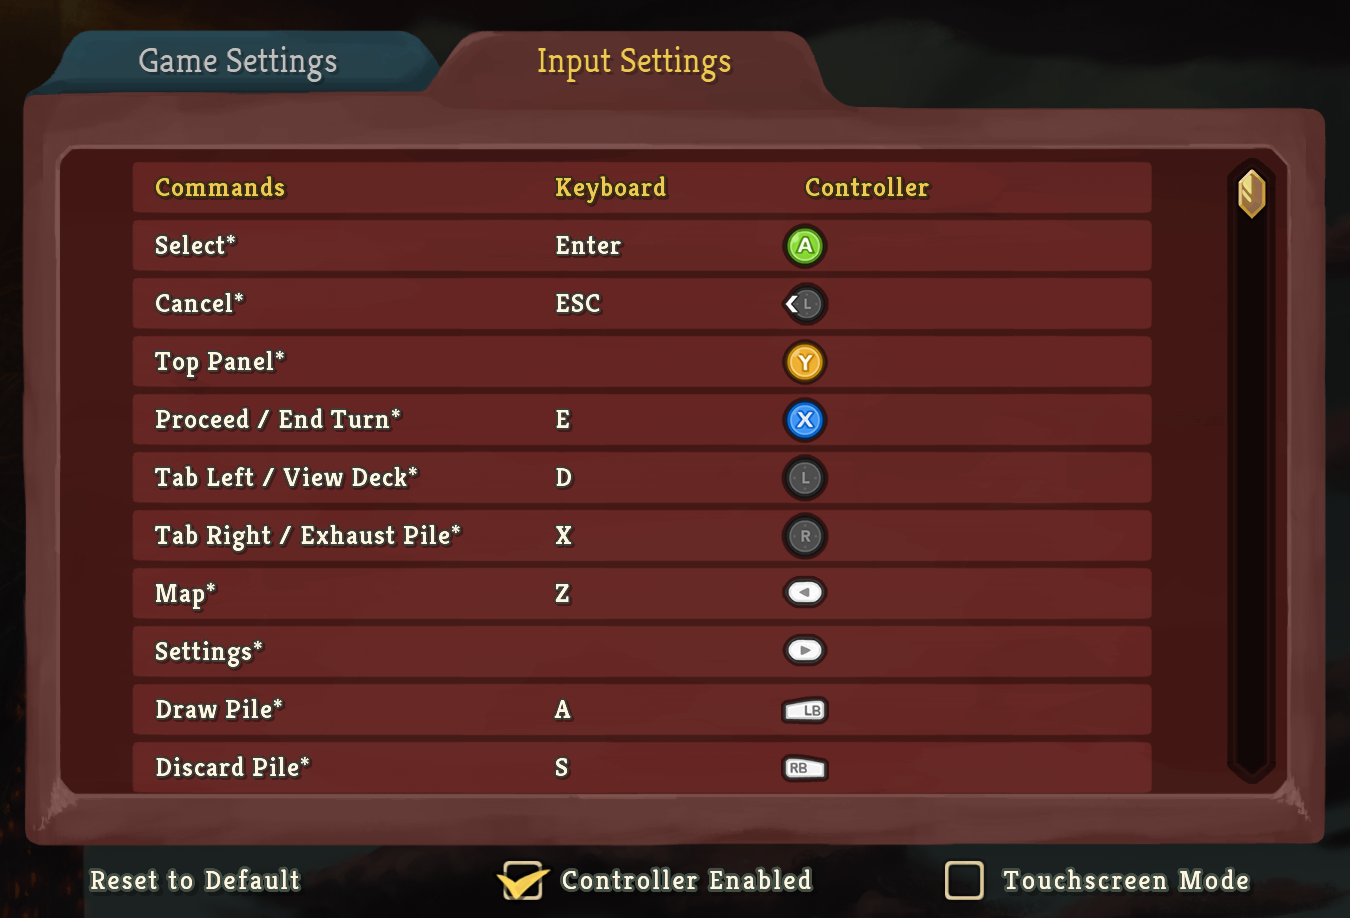
\includegraphics[scale=.25]{graphics/InputSettings1.PNG} & 
        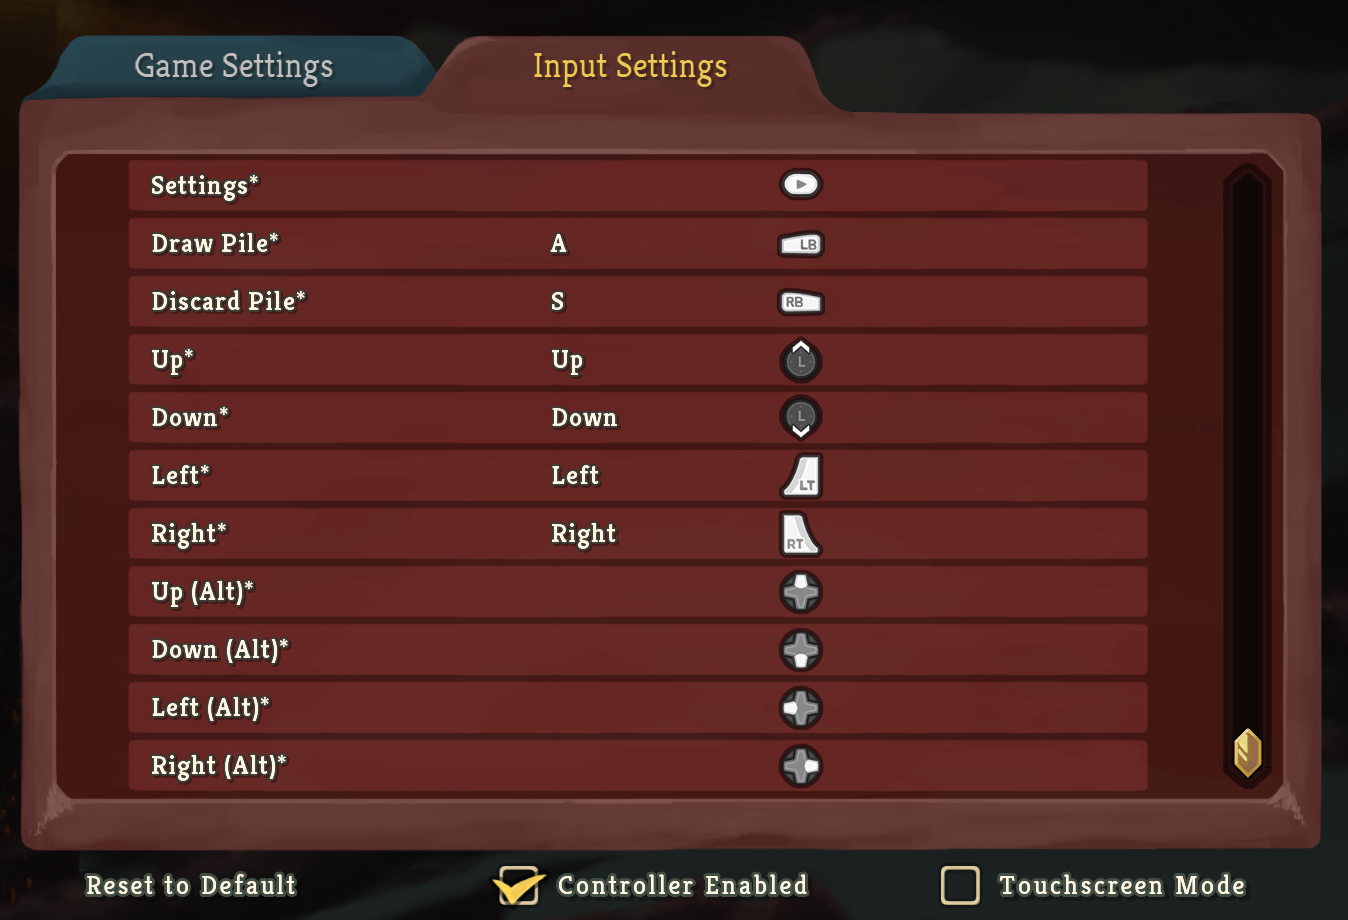
\includegraphics[scale=.25]{graphics/InputSettings2.PNG}
    \end{tabular}
    \caption{An example controller button layout.  }
    \label{fig: controller layout}
\end{figure}
\section{Basic strategies}
\begin{itemize}
    \item pathing
    \item removing, upgrading, and transforming
    \item event decisions
    \item potion use
    \item good cards and relics for each class
\end{itemize}
\section{Glitches and other exploits}\label{sec: glitches and exploits}
\subsection{Card skipping (Curse skip \& Bites skip)}\label{sub-sec: card skips}
Several events offer the player resources in exchange for a curse.  
In addition, other events such as  \textit{Vampires(?)}, add cards directly into the player's deck after certain selections.  
The player can also skip the curse obtained after opening a chest with Cursed Key.  
By entering a new map node before the completion of this animation, the player avoids adding the new card to their deck.  
Our writeup is based on Forgotten Arbiter's video tutorial (see \cite{ForgottenArbiterMoreGlitches}).  
\\

The most common way to do this is by mashing `select' on a controller while making the selection.  
Note that: 
\begin{itemize}
    \item 
        If the player skips curses, then  Omamori and Darkstone Periapt do not proc.  
    \item 
        If the player skips Bites at the \textit{Vampires(?)} event, then their Strike cards are still removed.  
\end{itemize}
See Figure \ref{fig: card skips} for screenshots of two useful card skips.  
\begin{figure}[h]
    \centering
    \begin{tabular}{c|c}
        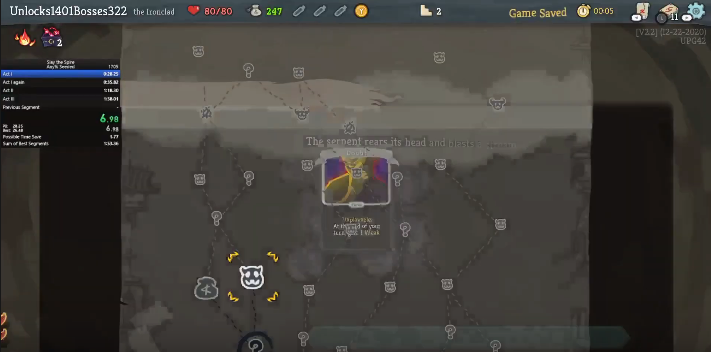
\includegraphics[scale=.3]{graphics/CurseSkip.png}
        & 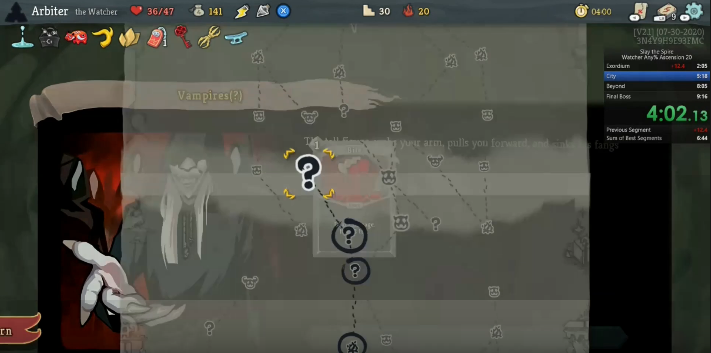
\includegraphics[scale=.3]{graphics/BitesSkip.png}
    \end{tabular}
    \caption{The screen just before entering a map node, skipping a Doubt or Bites.  }
    \label{fig: card skips}
\end{figure}
\subsection{Node buffering}\label{sub-sec: node buffering}
In this section, we will discussion glitches that involve ``buffering'' map nodes.  
When the player selects a map node (say, node \textbf{A}), the player enters node \text{A} only after a $1/4$ second-long screen transition.  
Since the timer only ticks while the map is on-screen, returning to the previous screen allows the player to make a variety of actions.  
\\

As we will see in Sections \ref{sub-sub-sec: 2-node} and \ref{sub-sub-sec: other applications}, it is possible for multiple timers to exist simultaneously.  
While the map is pulled up, all timers run simultaneously.  
When the first timer reaches $0$ seconds, the player is taken to the corresponding node.  
Returning to the map screen repeats this process.  
\\

\subsubsection{Necronomicurse skip and unlock farming}
The earliest major use of node buffering came during the \text{Cursed Tome} event when the player is offered the Necronomicurse.  
Our writeup is based on Forgotten Arbiter's video tutorials (see \cite{ForgottenArbiterGlitches} and  \cite{ForgottenArbiterMoreGlitches}).  \\

If the player proceeds through the event selections and sees the relic offered, they are able to select and enter nodes on the map without exiting the reward screen.  
If the Necronomicon is offered, the player can buffer the next map node, which takes them back to the reward screen.  
After taking the Necronomicon, the player pulls up the map and enters the node before the Necronomicurse enters their deck.  
See Figure \ref{fig: necro skip} for a screenshot which shows this glitch in action.  
\begin{figure}[h]
    \centering
    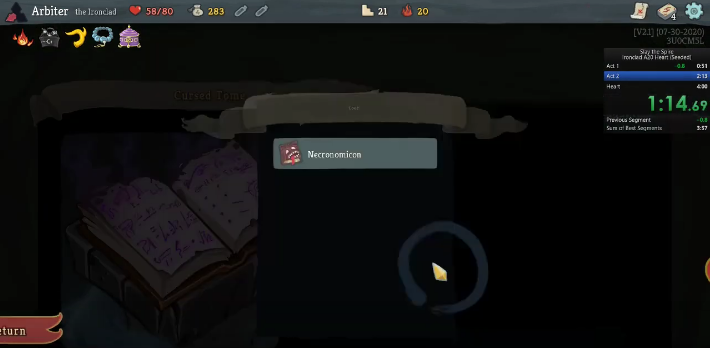
\includegraphics[scale = .3]{graphics/NecronomicurseSkip.png}
    \caption{Skipping the Necronomicurse using this method.  
    The circle indicates that a map node has been buffered by the player.  
    }
    \label{fig: necro skip}
\end{figure}
\\

When manually setting up a save setup, the player can use node buffering to add their current score to the metagame total and progress unlocks multiple times during one run.  
To do this, buffer entry into a node, but do not enter it.  
Open the settings menu and abandon the run.  
After advancing the post-run menu once, score will be tallied.  
The player may then open the map.  
Instead of taking the player to the next node, the player re-enters the post-run menu but can quit to the main menu.  
If the player continues the run, they may continue to accumulate and tally score.  
\subsubsection{$2$-node glitch}\label{sub-sub-sec: 2-node}
The player can visit $2$ nodes (or more, with very precise inputs) that are reachable from their current floor.  
This is especially useful ahead of treasure rooms and also when the player wishes to reach map nodes that are not on their desired path.  
Any animations, combats, and events from the first node can be interrupted by entering the second node.  
This provides an alternative method to prevent cards such as curses and Bites from being added to the player's deck (see Section \ref{sub-sec: card skips}).  
Additionally, if the player is fast enough and the first node is a combat, then Neow's Lament will not decrement.  
For a detailed video tutorial of this glitch, see \cite{ForgottenArbiterMoreGlitches}.  
\\

With node \text{A} buffered, the player pulls the map back up and select another node \textbf{B} before the node \textbf{A} timer completes.  
If performed correctly, the first timer completes and the player enters node \text{A} and takes any actions they desired.  
When the player re-enters the map, the next timer will tick and the player will then enter node \textbf{B}.  
To perform this glitch on \mk:  
\begin{itemize}
    \item 
        Enter the map screen without scrolling and locate nodes \textbf{A} and \textbf{B}.  
    \item 
        Click node \textbf{A} and press the `map' key to return to the current node screen.  
    \item 
        Mouse over the position of node \textbf{B}, pull up the map, and immediately click node \textbf{B}. 
\end{itemize}
To perform this glitch on \con: 
\begin{itemize}
    \item 
        Enter the map screen and locate nodes \textbf{A} and \textbf{B}.  
    \item 
        Select node \textbf{A} and press the `map' button to return to the current node.  
    \item 
        Pull the node back up, move the selection to node \textbf{B}, and select node \textbf{B}.  
        Recall from Section \ref{sec: input methods} that when the map is pulled up, the default selection is the middle-most, or right-middle node based on the parity of the number of nodes.  
\end{itemize}
To enter a third node \textbf{C} which is also reachable from the current node, they may repeat the action used to buffer node \textbf{B} before the node \textbf{A} timer completes.  

\subsubsection{Double bosses and other applications}\label{sub-sub-sec: other applications}
The player can use node buffering to achieve a variety of complex outcomes.  
Because of the technical precision required and the timeloss inherent in visiting extra floors, this is usually unhelpful in speedrunning.  
However for seeded runs and speedrun-adjacent challenge, they can be nonetheless useful.  
\\

The player may enter a boss combat and earn all associated rewards multiple times by buffering nodes.  
While typically this results in time loss, it can be helpful in seeded runs where the player has charges of Neow's Lament remaining or when the player is able to quickly defeat the boss.  
Unlike other map nodes, when the player selects ad boss combat node, they enter the boss combat immediately and without a timer.  
By buffering into $2$ or more rest site nodes, the player may, after completing their action at each rest site, return to the map and immediately select the boss combat node.  
After collecting rewards, the player may reopen the map screen and repeat this process at the next rest site they buffered.  
\\

By buffering map nodes, the player may visit a complicated ``branching'' path.  
To do this, the player buffers entry into $2$ or more nodes from their current positions.  
After entering the first buffered node, they may then buffer multiple nodes from their current nodes.  
Since all timers run simultaneously while the map screen is open, these new timers will expire one-by-one \textit{after} the timers from the previously buffered nodes expire.  
This can be useful when the player wishes to visit two or more nodes that are not on their desired route.  
For example, the player may wish to spend a charge of Neow's Lament on an Elite combat (node \textbf{A}) and visit a Shop (node \textbf{C}), but then continue from a node (node \textbf{D}) other than the shop node which was reachable from node \textbf{B}.  \\

Alternatively, you may think of the route taken along a branching path as the order given by a \textit{breadth-first search} (see Figure \ref{fig: BFS tree}).  
When the player buffers nodes from their current node, they effectively add each buffered node to the back of a queue.  
When the player pulls up the map long enough for a timer to reach $0$ seconds, they then travel to the first node in queue.  
Note that the order of node traversal need not be represented purely by a tree.  
If the player map (viewed upside-down) is represented by Figure \ref{fig: BFS tree} but instead node $8$ also connects to node $11$, then the player may visit node $11$ twice.  
\begin{figure}[h]
    \centering
    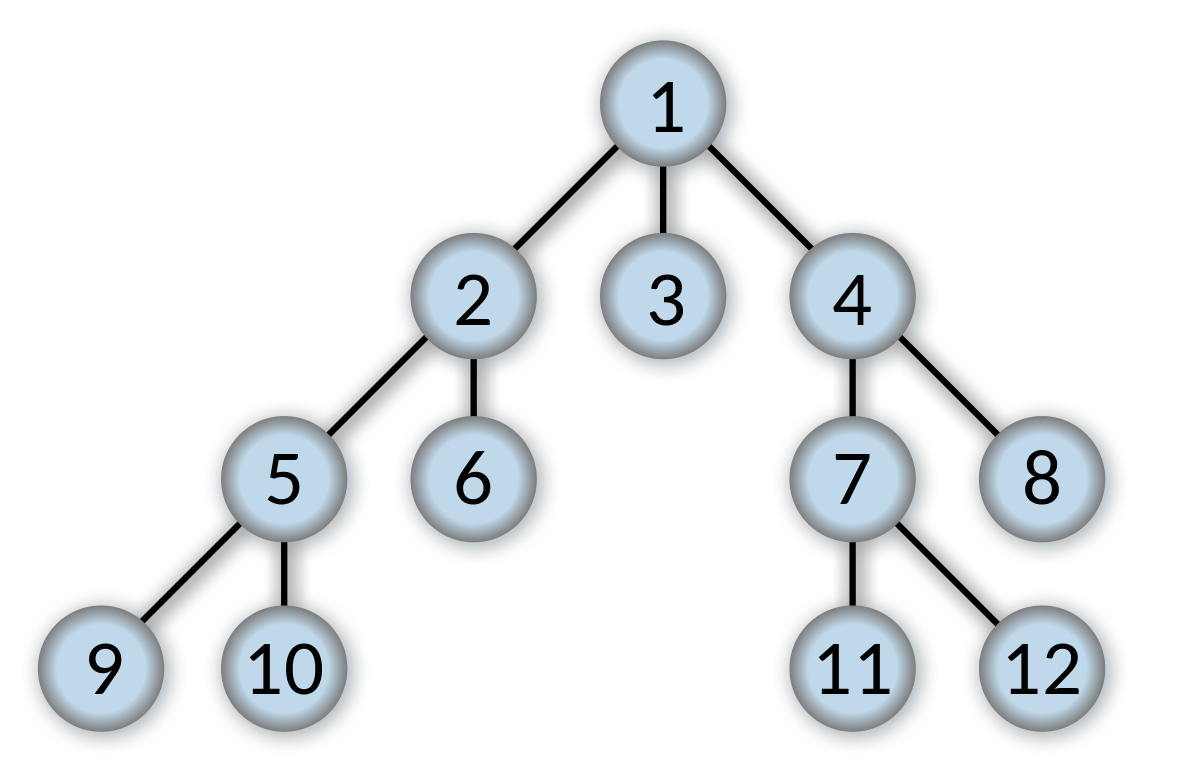
\includegraphics[scale=.1]{graphics/BFSTree.png}
    \caption{A breadth-first ordering on a tree.  }
    \label{fig: BFS tree}
\end{figure}
\subsection{Pandora's Box (and Calling Bell) glitch}\label{sub-sec: pandora's box glitch}
By far, this is the most impactful easy-to-perform glitch for new \sts~speedrunners to learn.  
After taking Pandora's Box, the player is able to remove all Strike and Defend cards without adding the new `transformed' cards.  
Our writeup is based on Forgotten Arbiter's video tutorial (see \cite{ForgottenArbiterMoreGlitches}).  
\\

Normally when the player transforms cards, he selected card(s) are instantly removed from the deck and a brief animation begins which adds the new card(s) to their deck.  
When the player obtains Pandora's Box, their Strike and Defend cards are immediately removed, but instead of an animation, a brief delay takes place and the new cards appear on a screenlayer.  
When the player selects `confirm' on the screenlayer, these cards are added to their deck.  
The player can prevent adding the cards from the screenlayer to their deck using either of the game's legal input methods: 
\begin{itemize}
    \item 
        On \mk, no precise timing is needed.  
        The player takes advantage of the way the game handles screen layers.  
        After the card transformation screenlayer appears, the player must enter the settings menu, select `abandon run', and press the `cancel' key (by default, \textrm{ESC}) twice.  
        This removes the screenlayer and the player may then select `confirm' to proceed to the next Act.  
    \item 
        The method on \con, requires either precise timing or mashing and only works when taking Pandora's Box on the boss relic reward screen.  
        Here, the player is able to  `confirm' their boss relic selection and enter the next Act in a narrow frame-window between after the transformed card screenlayer appears, but before the new cards can be `confirmed'.  
        To proceed, simply pull up the map and select the desired node. This also skips the $5$-second map scroll, so during unseeded runs, the player must manually scroll up to plan their route through the next Act.  
\end{itemize}
See Figure \ref{fig: Pandora's Box glitch} to see this glitch in action.  
\begin{figure}[h]
    \centering
    \begin{tabular}{c|c}
        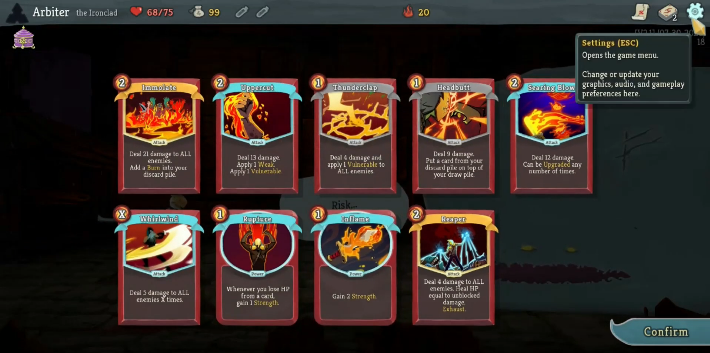
\includegraphics[scale=.3]{graphics/PandorasBoxGlitchMK.png} & 
        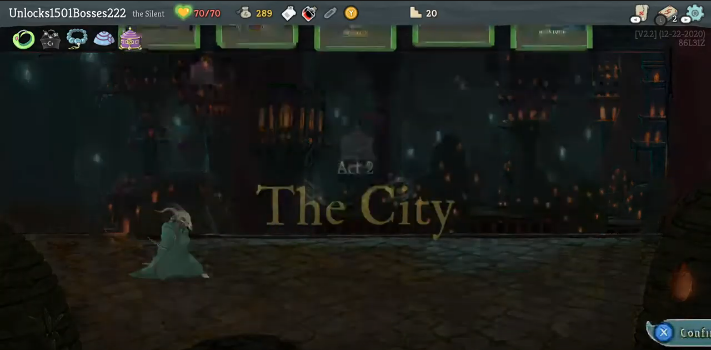
\includegraphics[scale=.3]{graphics/PandorasBoxGlitchCON.png}
    \end{tabular}
    \caption{Skipping the cards from Pandora's Box on each input method.  }
    \label{fig: Pandora's Box glitch}
\end{figure}
The player can also skip the curse after taking the Calling Bell relic in a similar fashion.  
With \mk, the player skips a screenlayer which normally adds the Curse of the Bell to their deck and enters the relic reward screen.  
On \con~however, the player is not given access to the relics given by Calling Bell and they are only given the opportunity to skip the curse and the map scroll.  
\subsection{Smoke bomb glitch}\label{sub-sec: smoke bomb glitch}
Although the player is not able to use a smoke bomb during a boss combat, there is a glitch that allows the player to skip a boss combat and still receive the usual rewards.  
Our writeup is based on Forgotten Arbiter's video tutorial (see \cite{ForgottenArbiterMoreGlitches}).  
\\

When the player uses a smoke bomb, a $2.5$ second timer begins.  
The timer does not tick during reward screens and or on the map screen.  
If the player is in combat when the timer reaches $0$ seconds, then the combat immediately ends.  
The player does not receive rewards from the combat where the smoke bomb was played, but will receive rewards if the timer ends during another combat.  
\\

To perform this glitch, the player needs to end a combat before a smoke bomb timer reaches $0$ seconds.  
This can be done in many ways, such as: 
\begin{itemize}
    \item 
        Throwing a smoke bomb immediately after ending a turn where lighting orbs deal lethal damage.  
    \item 
        Throwing a smoke bomb immediately before playing a lethal card that has a short animation.  
    \item 
        Throwing a smoke bomb during the animation of a lethal card if the animation is long.  
\end{itemize}
In certain scenarios, it may be easier to perform this glitch on \con~instead of \mk.  
See Figure \ref{fig: smoke bomb glitch} for a few instances of the smoke bomb glitch in action.  
\begin{figure}[h]
    \centering
    \begin{tabular}{c|c}
        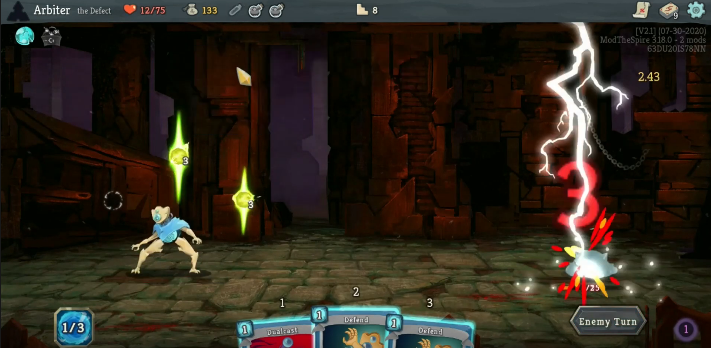
\includegraphics[scale=.3]{graphics/SmokeBomb1.png} & 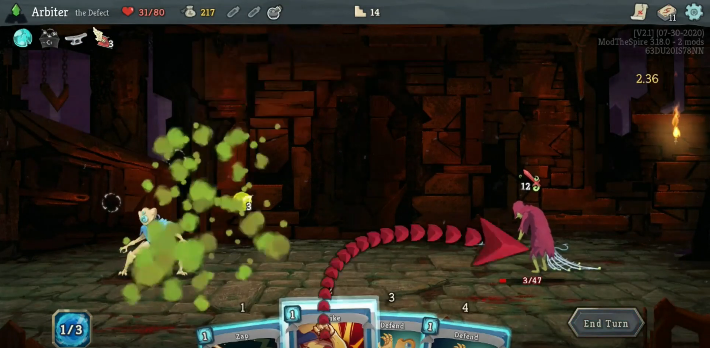
\includegraphics[scale=.3]{graphics/SmokeBomb2.png}
        \\
        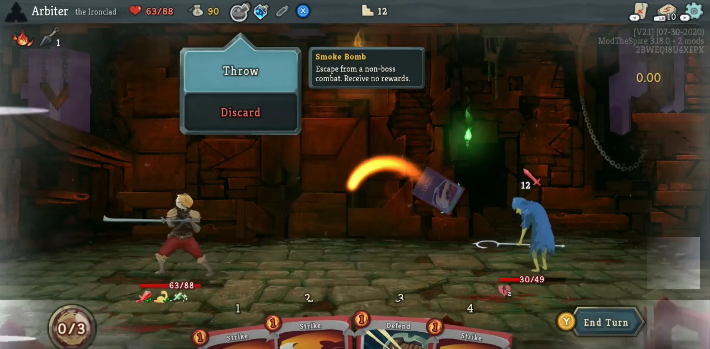
\includegraphics[scale=.3]{graphics/SmokeBomb4.png} &
        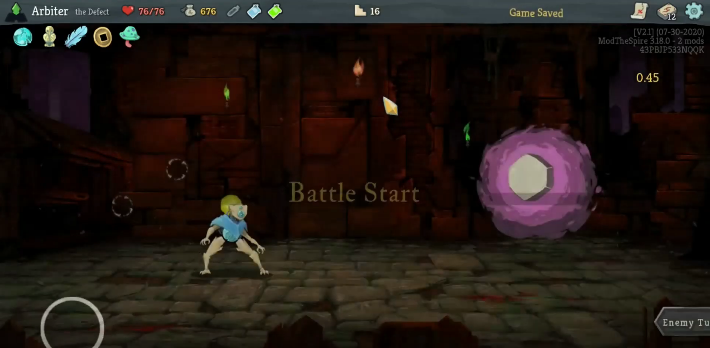
\includegraphics[scale=.3]{graphics/SmokeBomb5.png} \\ 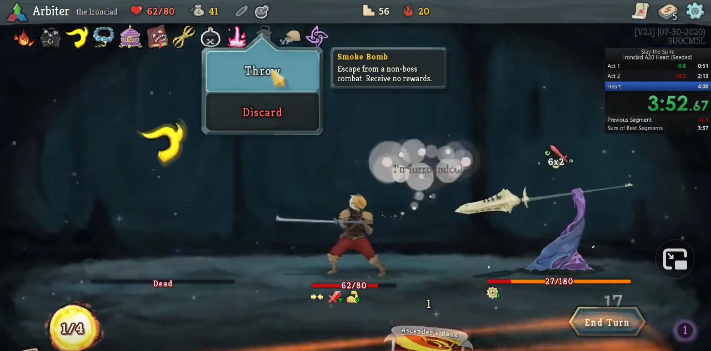
\includegraphics[scale=.3]{graphics/SmokeBomb6.png}
        &
        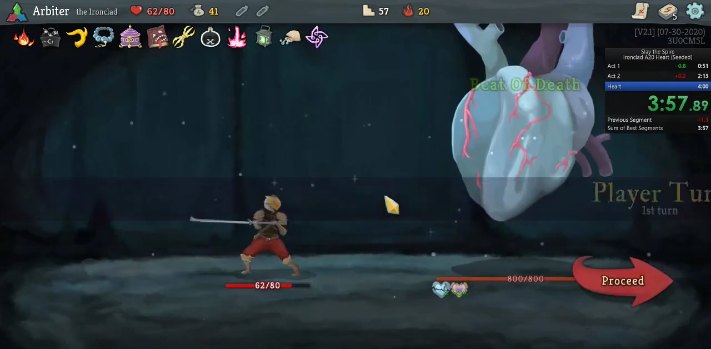
\includegraphics[scale=.3]{graphics/SmokeBomb7.png} 
    \end{tabular}
    \caption{Setting up the smoke bomb glitch and skipping bosses.  }
    \label{fig: smoke bomb glitch}
\end{figure}
\subsection{Correlated randomness}\label{sub-sec: RNG}
Certain calls to the game's pseudorandom number generator (determined by the run's seed) are reused.  
See Forgotten Arbiter's post \cite{ForgottenArbiterCorrelatedRandomness} for a more detailed description.  
\\

Most practical is way that the game generates the outcome of a ? node.  
\begin{itemize}
    \item 
        Explain how event RNG gets updated after visiting a ? node.  
    \item 
        Explain how ``shrine'' events can guarantee, or nearly guarantee, that the next ? node is a combat.  
    \item 
        Cultist? 
\end{itemize}


\newpage
\bibliography{mybib}
\bibliographystyle{plain}


\end{document}

